\chapter{From ZDRa to General Proof Sketch}
\label{ch:skeletons}

The skeletons described in this chapter are automatically generated if the specification passes the \gls{zdra} check. Section \ref{sec:zdra2gen} describes the general proof skeleton. Which uses the graphs generated in the \gls{zdra} to provide the order the instaces should go to into any theorem prover. Section \ref{chap:gpsa2isa} then explains how a general proof skeleton can be automatically translated into a skeleton in Isabelle format automatically. In section \ref{sec:isa2ful} we describe how the Isabelle Skeleton can be used to fully prove a formal specification which requires two steps, the first is an automatic step to fill in the Isabelle skeleton and the final step is up to the user to prove the lemma's and properties of the specification.

\section{What is a General Proof Sketch}
\label{sec:zdra2gen}

When checking for ZDRa correctness the program adds all the annotated chunks into a dependency graph and a GoTo graph. Both these graphs are directed graphs.

We then run an algorithm on the GoTo graph to generate a proof skeleton. Figure \ref{fig:code} shows part of the code in generating this proof sketch.

\begin{itemize}
\item \textit{allnodes}, is a set of all the instances labelled by the user of a specification in ZDRa.

\item \textit{fromnodes}, is a set containing all the nodes which are dependent on another instance.

\item \textit{tonodes}, is a set containing all the nodes which have some other nodes dependent on them.
\end{itemize}

\begin{figure}[H]
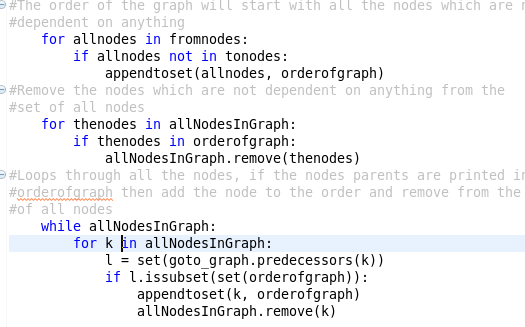
\includegraphics[scale=0.5]{Figures/skeleton/code.png}
\caption{Part of the algorithm to create a proof sketch.}
\label{fig:code}
\end{figure}

\section{Creating the Graph}

Here we show how a Proof skeleton is calculated using the Goto graph created when running the ZDRa check on a specification.

\begin{figure}[H]
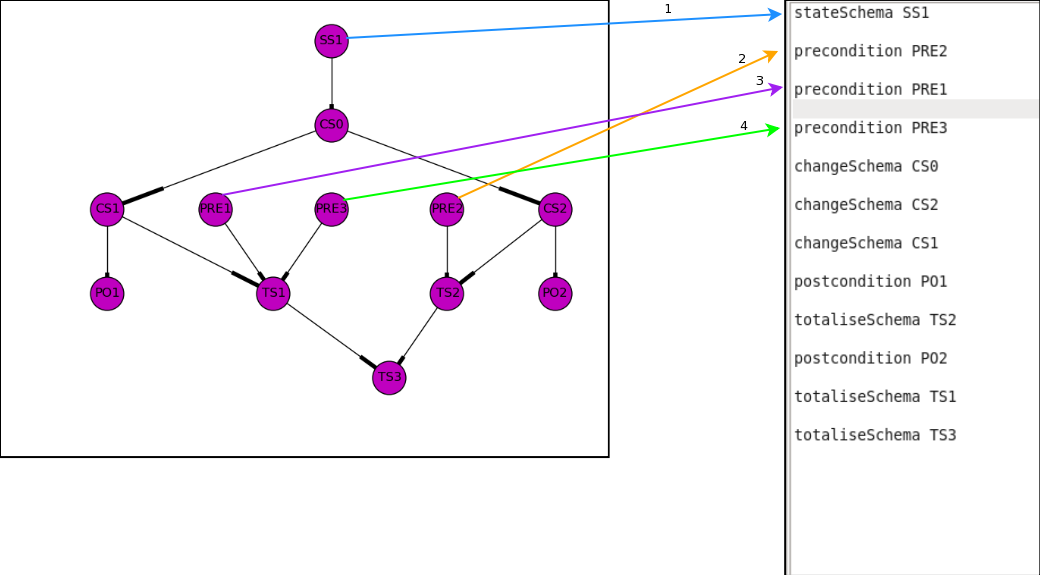
\includegraphics[scale=0.3]{Figures/skeleton/1.png}
\caption{GoTo graph and proof skeleton of vending machine step 1.}
\label{fig:1}
\end{figure}

First of all the program looks at all the nodes of the GoTo graph and prints out all the nodes which are not dependent on anything. That is, they may have successors but they have no predecessors, they do not use or need anything else and can stand by themselves. These nodes can be printed in any order, so in diagram \ref{fig:1} we see that we have SS1, PRE1 PRE2 and PRE3 all printed.

\begin{figure}[H]
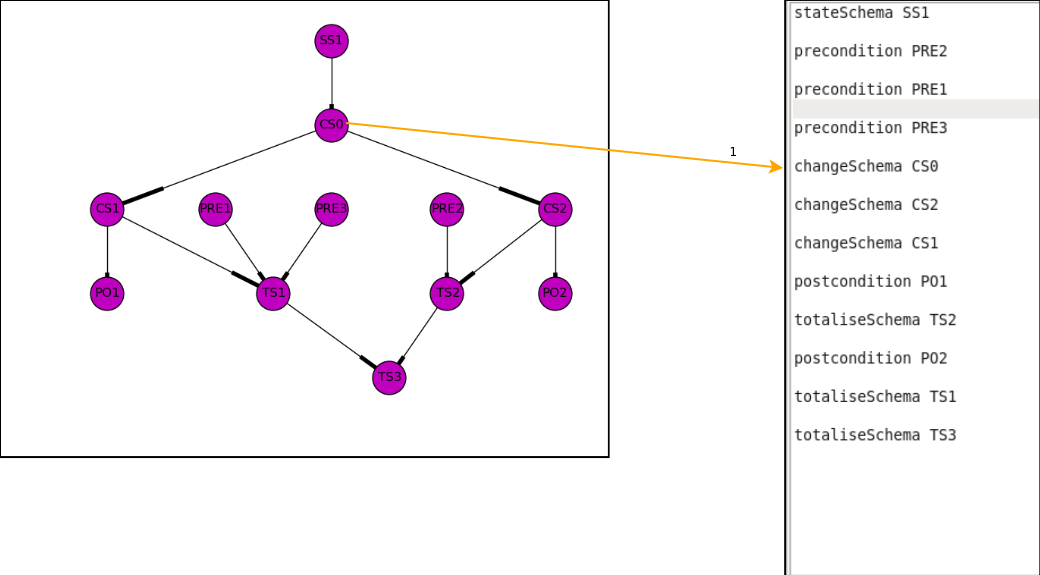
\includegraphics[scale=0.3]{Figures/skeleton/2.png}
\caption{GoTo graph and proof skeleton of vending machine step 2.}
\label{fig:2}
\end{figure}

The next part of the algorithm checks whether there exists a node in the GoTo graph where all of its parents are printed out in the proof skeleton. Figure \ref{fig:2} shows that the next node to be in the proof skeleton is CS0. 

\begin{figure}[H]
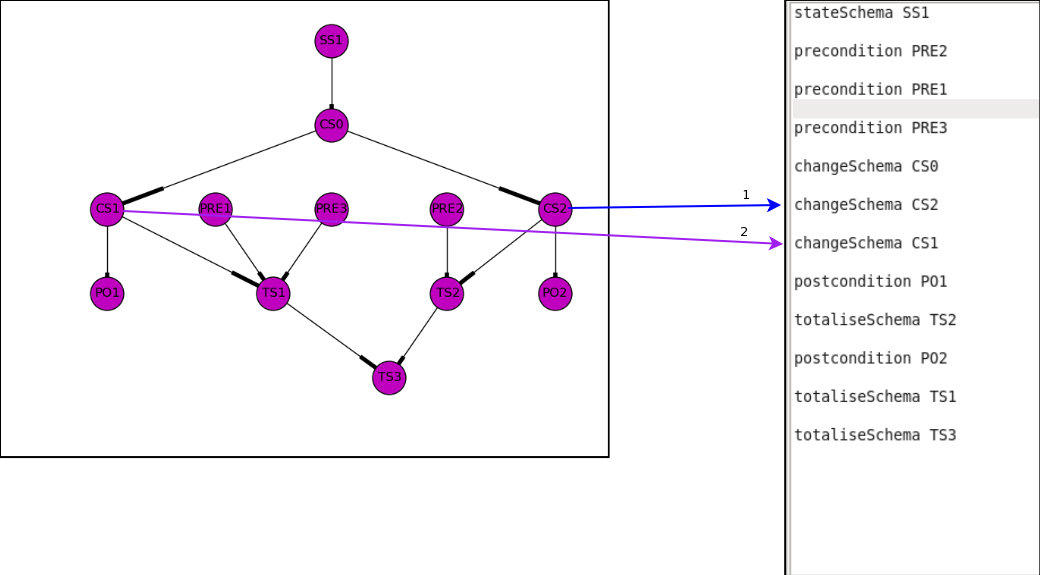
\includegraphics[scale=0.3]{Figures/skeleton/3.png}
\caption{GoTo graph and proof skeleton of vending machine step 3.}
\label{fig:3}
\end{figure}

The next part we see that after CS0 is added to the proof skeleton then both CS1, and CS2 can be added. This is shown in figure \ref{fig:3}.

\begin{figure}[H]
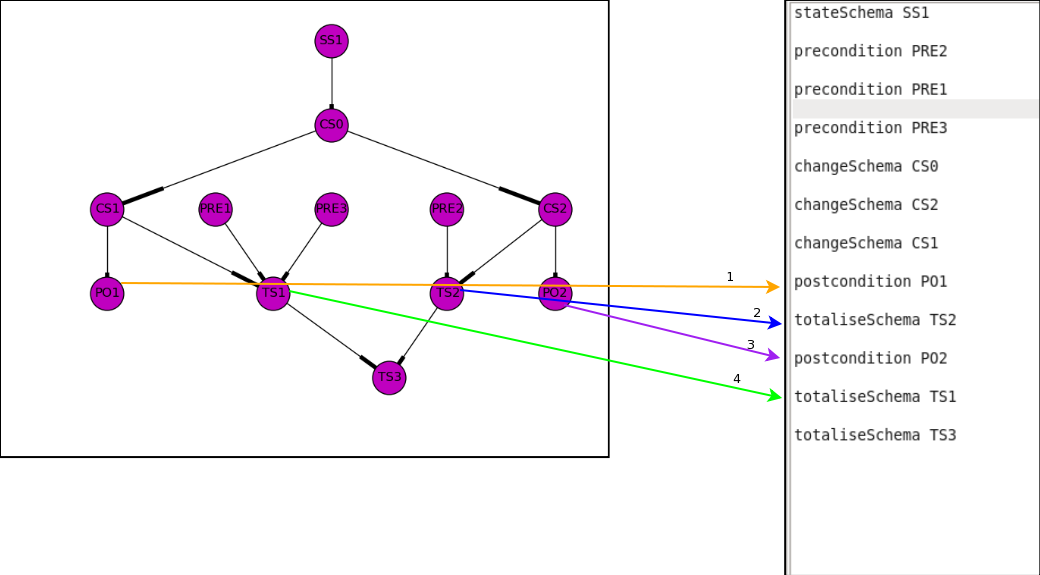
\includegraphics[scale=0.3]{Figures/skeleton/4.png}
\caption{GoTo graph and proof skeleton of vending machine step 4.}
\label{fig:4}
\end{figure}

Figure \ref{fig:4} shows the next stage of adding nodes to the Proof Skeleton. Since CS1 and CS2 are now added to the proof skeleton then the next row of nodes can be added. Since PO1 only had one parent (CS1) it is added first, PO2 also had one parent (CS2) it is added second. The others had more parents which are already in the proof sketch so they are added next randomly.

\begin{figure}[H]
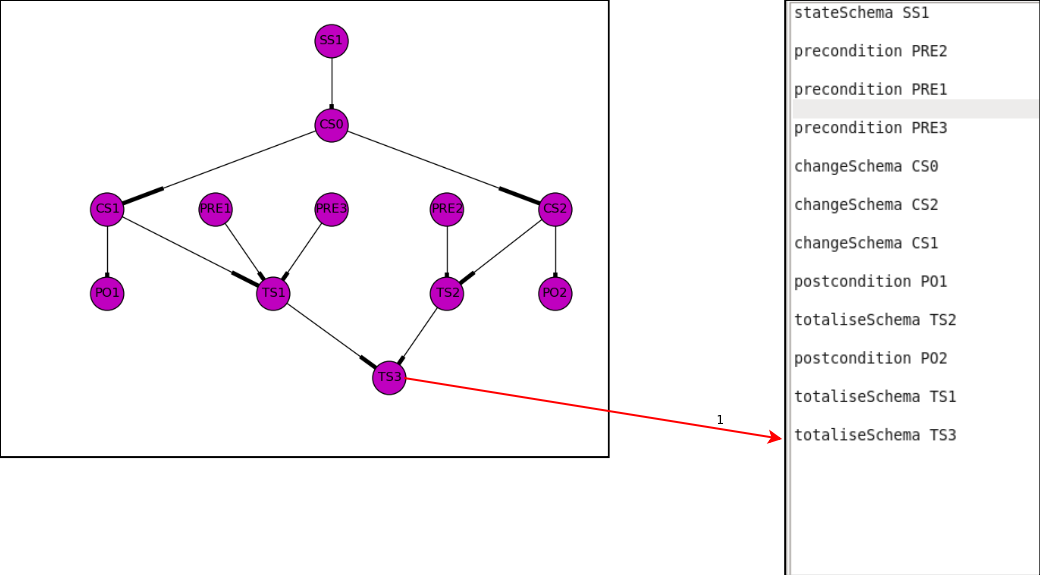
\includegraphics[scale=0.3]{Figures/skeleton/5.png}
\caption{GoTo graph and proof skeleton of vending machine step 5.}
\label{fig:5}
\end{figure}

We come to the final stage of the dependency graph, when all the nodes are in the dependency graph except for one which is added to the end.

\section{Proof Obligations}

There are many properties one may wish to prove about their specification. These certain properties are called proof obligations. Proof obligations for formal notations are an entire research area in their own right. However as the \gls{zmath} framework concentrates on giving the novice an idea of how to prove their specification we will focus on checking the specification for consistancy. Using the description in \cite{DBLP:conf/icsea/WenMZ06}, checking the specification is consitant can fall under two categories:

\begin{itemize}
\item POb1, Feasability of an operation
\item POb2, Other specific proof obligation for the chosen specification
\end{itemize}

We use the syntax \textit{Context} $\vdash$ \textit{predicate} taken from the paper to define the proof obligations.

\subsection{POb1, Proof Obligation type 1}

\begin{defin}\label{defa}POb1\\

$Context \vdash \exists var, var' \bullet SI\# \land SI\#' \land PRE\# \land PO\#$ \\

\noindent where var and var' are the variables and variables' used in the schema with their types, SI\# is the state Invariants of the specification, SI\#' is the state invariants prime in the specification, PRE\# is the precondition of the schema, PO\# is the post operation of the schema and \# is some arbitary number.
\end{defin}

POb1 shows the feasability of an operation. When an operation can transfor a state to another state in the state space (a $\Delta$ schema). If an operation is feasible, the preconditional state and postconditional state should satisfy the state invariants of the specification.

Again by using the ModuleReg specification we can see a proof obligation is needed when adding a student doesnt change the state invariants of the specification.

\begin{verbatim}
lemma AddStudentDoesntChangeSI:
"(\<exists> taking taking'  :: (PERSON * MODULE) set.
 \<exists> degModules degModules':: MODULE set.
 \<exists> students students':: PERSON set.
  \<exists> p :: PERSON.
(students' = students \<union> {(p)}) 
\<and> (taking' = taking)
\<and> (degModules' = degModules)
\<and> (Domain taking \<subseteq> students)
\<and> (Range taking \<subseteq> degModules)
\<and> (Domain taking' \<subseteq> students')
\<and> (Range taking' \<subseteq> degModules')
) "
\end{verbatim}

The ZDRa syntax of this proof obligation would be :

\begin{verbatim}
lemma AddStudentDoesntChangeSI:
" \<exists> (*CS1_variables :: CS1_TYPES*).
(PRE1)
\<and> (PO1)
\<and> (SI1)
\<and (SI1')"
\end{verbatim}

In this property we check that the preconditional state and post conditional state of the operational schema still hold the state invariants and prime state invariants. The ZDRa syntax of the proof obligation stays that there exists some variables of the operational schema where the precondition (PRE1) postCondition (PO1) stateInvariants (SI1) and stateInvariants prime all hold.

\subsection{POb2, Proof Obligation type 2}

As POb2 are any other relevent properties users wish to prove about the specification we can not formally define it. However an example would be if there existed a specification where an operator which added a member to a club and then removed a member from the club. Then the amount of members should be the same after both operators have completed the task.

One such example is in the ModuleReg specification the RegForModule schema postcondition shows that \verb|(taking' = taking ∪ {(p, m)}) | therefore if this were to happen then we should make sure that \verb|taking'| is not empty after the operation. This proof obligation is very specific to the ModuleReg specification and the user would need to write and check this themselves. To do such we have the following lemma:

\begin{verbatim}
lemma notEmpty:
"(taking' = taking \<union> {(p,m)}) 
\<longrightarrow> (taking' \<noteq> {})"
\end{verbatim}

Where the name of the lemma is \verb|notEmpty| then the postOperation of the ChangeSchema is \verb|(taking' = taking \<union> {(p,m)}) | then checking that the set is not empty follows the right arrow \verb|(taking' \<noteq> {})|.

POb1 can be automate. Since POb2 is specification specific, each user will need to define these themselves if they so wish.

\subsection{Proof Obligations in the General Proof Skeleton}

Since the POb2 are specific to the specification only POb1 are automatically added. They are generated as `\emph{lemma's}' in the general proof skeleton. 

\begin{figure}[H]
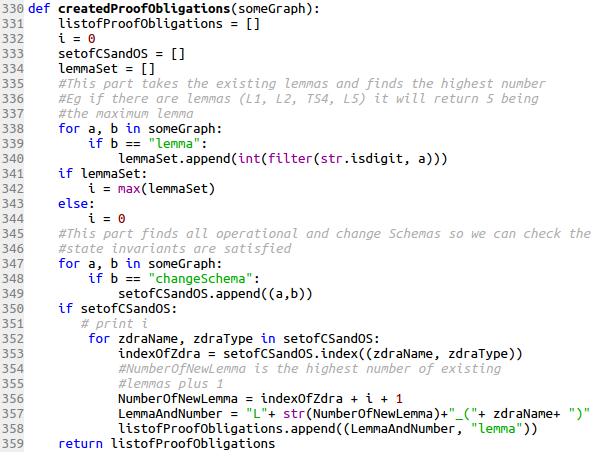
\includegraphics[scale=0.6]{Figures/skeleton/pobcode.png}
\caption{Part of the algorithm to create Proof Obligation ZDRa names.}
\label{fig:codepob}
\end{figure}

The proof obligations which check that changeSchema's and outputSchema's follow the stateInvariants are added to the original general proof skeleton. The general proof skeleton starts of with being an ordered list (GPSaOL), then the algorithm for generating a list of proof obligations is run and added to the original proof skeleton. Figure \ref{fig:codepob} shows the algorithm which creates the ordered list of proof obligations.

Lines 338-344 find all the existing lemma's in the \gls{gpsol} and sets \emph{i} to be the highest number. For example if there are existing lemmas in \gls{gpsol} (L1, L2, L3), then \emph{i} becomes 3. If there are no existing lemmas in \gls{gpsol} then \emph{i} stays as 0. Lines 347-250 take all the elements which are \emph{changeSchema} instances and adds them to a list of \emph{setCSandOS}. Then lines 350-359 loops through all the changeSchema's, takes the \gls{zdra} name, add's L + a number + \gls{zdra} name and adds it to the \emph{listOfProofObligations}.

\paragraph{For Example}

if we had the following \gls{gpsol}: \\
\noindent [(SS1, stateSchema), (IS1, initialSchema), (CS1, changeSchema), (CS2, changeSchema), (TS1, totaliseSchema)] \\
Then in this case:
\begin{itemize}
\item lemmaSet = []
\item i = 0
\item setofCsandOs = [(CS1, changeSchema), (CS2, changeSchema)]
\end{itemize}

Then for each element in setofCsandOs we would add the new elements (L1\_CS1, lemma) and (L2\_CS2, lemma) to the ordered list \emph{listOfProofObligations}.

The new \gls{gpsol} would then become [(SS1, stateSchema), (IS1, initialSchema), (CS1, changeSchema), (CS2, changeSchema), (TS1, totaliseSchema), (L1\_CS1, lemma) and (L2\_CS2, lemma)]

If for example the original \gls{gpsol} was \\
\noindent [(SS1, stateSchema), (IS1, initialSchema), (CS1, changeSchema), (CS2, changeSchema), (TS1, totaliseSchema), (L1, lemma), (L2, lemma)]\\
Then then new proof obligation lemmas would be (L3\_CS1, lemma) and (L4\_CS2, lemma) as we would already have L1 and L2.

\begin{figure}[H]
\centering
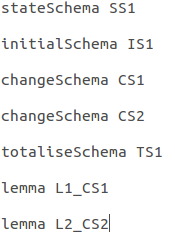
\includegraphics[scale=0.5]{Figures/skeleton/proofskeletonwithpo.png}
\caption{Example of a General Proof Skeleton with lemma's.}
\label{fig:gpswithpo}
\end{figure}

An example of a General Proof Skeleton with added proof obligations is shown in Figure \ref{fig:gpswithpo}. The changeSchema's in this specification are CS1 and CS2. Therefore to make sure the changeSchemas do not change the state of the specification and comply with the state invariants the two lemma's L1\_CS1 and L2\_CS2 have been added.

\subsubsection{Proof Obligations in specification examples}
Since the vending machine specification (appendix \ref{app:vm2}) doesn't have any stateInvaritants then the \gls{gps} will not have any added proof obligations to check for consistance. That is we can't check that the postconditions do not change the state if the state has no restrictions. However the birthdaybook example (appendix \ref{app:bb3}) does have stateInvariants. Therfore we must add properties to check that any changeSchema's follow the state restrictions. Part of the birthdaybook \gls{gps} is shown in figure \ref{fig:bbgps}. Since there are stateInvariants (SI1) and a changing state Schema (CS1) then the proof obligation \texttt{L1\_(CS1)} has been added to the \gls{gps}.

\begin{figure}[H]
\begin{verbatim}
stateSchema SS1 
stateInvarients SI1 
initialSchema IS1 
postcondition PO2 
outputSchema OS1 
precondition PRE2 
changeSchema CS1 
totaliseSchema TS1 
.......
lemma L1_(CS1) 
\end{verbatim}
\caption{Part of the GPSa for the birthdayBook example. (Full version shown in appendix \ref{app:bb3}) \label{fig:bbgps}}
\end{figure}

\section{Conclusion}
\label{sec:skeletonsConclusion}

This chapter describes how the \gls{zdra} program uses the GoTo graph to generate a general proof skeleton (step 2$\rightarrow$3 in figure \ref{fig:steps}). The general proof skeleton is an automatically generated .txt file which displays the order in which this instances must go in a theorem prover to be logically correct. This chapter gives a basic understanding of proof obligations for Z and examples which proof obligations are automatically generated when translating Z specifications into Isabelle. We give a formal definition of the proof obligation to check for consistancy of the state invariants and show an example. The next chapter describes how the general proof skeleton is translated into Isabelle syntax.